\documentclass[conference]{IEEEtran}
\IEEEoverridecommandlockouts
% The preceding line is only needed to identify funding in the first footnote. If that is unneeded, please comment it out.
\usepackage[utf8]{inputenc}
\usepackage[brazilian,english]{babel}
\usepackage{cite}
\usepackage{amsmath,amssymb,amsfonts}
\usepackage{algorithmic}
\usepackage{graphicx}
\usepackage{textcomp}
\usepackage{xcolor}
\usepackage[most]{tcolorbox}
\usepackage{url}
\def\UrlBreaks{\do\/\do-}
\def\BibTeX{{\rm B\kern-.05em{\sc i\kern-.025em b}\kern-.08em
    T\kern-.1667em\lower.7ex\hbox{E}\kern-.125emX}}
\begin{document}

\title{Experimental Evaluation of the Capability of LLMs in Solving Problems in the Programming Category of the Brazilian Olympiad in Informatics}

\author{\IEEEauthorblockN{1\textsuperscript{st} Victor Hugo S. Ângelo}
\IEEEauthorblockA{\textit{Institute of Computing} \\
\textit{Federal University of Alagoas (UFAL)}\\
Maceió, AL, Brazil \\
vhsa@ic.ufal.br}
\and
\IEEEauthorblockN{2\textsuperscript{nd} Ricardo Vinicius A. Fernandes}
\IEEEauthorblockA{\textit{Institute of Computing} \\
\textit{Federal University of Alagoas (UFAL)}\\
Maceió, AL, Brazil \\
rvaf@ic.ufal.br}
\and
\IEEEauthorblockN{3\textsuperscript{th} Lucas Heron S. Anchieta}
\IEEEauthorblockA{\textit{Institute of Computing} \\
\textit{Federal University of Alagoas (UFAL)}\\
Maceió, AL, Brazil \\
lhsa@ic.ufal.br}
\and
\IEEEauthorblockN{4\textsuperscript{rd} Matheus Ryan S. Nascimento}
\IEEEauthorblockA{\textit{Institute of Computing} \\
\textit{Federal University of Alagoas (UFAL)}\\
Maceió, AL, Brazil \\
mrysn@ic.ufal.br}
\and
\IEEEauthorblockN{~~~~~~~~~~~~~~~~~~~~~~~~~~~~~~~~~~~~~~~~~}
\IEEEauthorblockA{~~~~~~~~~~~~~~~~~~~~~~~~~~~~~~~~~~~~~~~~~ \\
~~~~~~~~~~~~~~~~~~~~~~~~~~~~~~~~~~~~~~~~~ \\
~~~~~~~~~~~~~~~~~~~~~~~~~~~~~~~~~~~~~~~~~ \\
~~~~~~~~~~~~~~~~~~~~~~~~~~~~~~~~~~~~~~~~~}
\and
\IEEEauthorblockN{5\textsuperscript{th} Evandro de B. Costa}
\IEEEauthorblockA{\textit{Institute of Computing} \\
\textit{Federal University of Alagoas (UFAL)}\\
Maceió, AL, Brazil \\
evandro@ic.ufal.br}
}

\maketitle

\begin{abstract}
Large Language Models (LLMs) have demonstrated increasing capabilities in code generation, yet evaluating their performance in scenarios requiring complex algorithmic reasoning remains an open challenge. Competitive programming rigorously tests Artificial Intelligence by demanding semantic disambiguation, abstract computational modeling, and code optimization under strict time and memory constraints. This article presents a comprehensive experimental evaluation of the capacity of LLMs to solve programming problems within the context of the Brazilian Olympiad in Informatics (OBI). To this end, we developed an automated experimental environment using a curated dataset of OBI problems, categorized by difficulty and algorithmic scope, integrated with an automated judge for real-time code execution and validation. The benchmarking encompassed multiple state-of-the-art models, analyzing metrics such as correct resolution rate, compilation success, and performance across difficulty tiers. Results reveal that while models achieve high mastery in basic-level problems, they face significant degradation in advanced topics involving dynamic programming and graphs. Furthermore, the investigation demonstrates that multi-agent collaborative approaches outperform single-agent configurations, and that few-shot prompting is essential to align model outputs with strict formatting and I/O constraints. By mapping the current boundaries of these tools, this study provides a solid foundation for their future integration as pedagogical support in competitive programming education.
\end{abstract}

\begin{IEEEkeywords}
Large Language Models, Competitive Programming, Brazilian Olympiad in Informatics, Code Generation, Educational Support.
\end{IEEEkeywords}

\section{Introduction}\label{sec:introduction}

Automatic programming problem solving is one of the longstanding challenges in Artificial Intelligence. Unlike conventional software engineering tasks, competitive programming requires sophisticated skills from software developers. The AI agent must be able to interpret ambiguous problem statements, requiring semantic disambiguation, extract implicit requirements, perform abstract computational modeling, and design optimized algorithms under constraints related to computational cost, including execution time and memory. In the Brazilian computing educational scenario, the Brazilian Olympiad in Informatics (OBI) stands out as one of the instruments fostering these skills, challenging students to solve highly complex programming problems under strict time and memory constraints.

In parallel, the emergence and rapid evolution of Large Language Models (LLMs) have transformed the fields of software engineering and artificial intelligence, demonstrating important capabilities in automatic code generation and the translation of natural language requirements into programming languages. However, the application of these tools in competitive programming contexts still presents significant performance gaps. In these scenarios, the problem statements frequently require deep semantic interpretation and the construction of complex chains of reasoning, as well as the employment of advanced techniques such as dynamic programming and graph theory. Although national and international studies investigate the capability of LLMs in problem-solving across various contexts and domains \cite{chen2021evaluating, mendonca2024evaluating, viegas2025assessing, huang2024competition, zheng2025livecodebench, li2024evaluating, almeida2023bluex}, there is still a lack of experimental evidence regarding the behavior of these tools when faced with problems located in competitive olympiads, such as those of the OBI.

Competitive programming emerges as a rigorous benchmark to evaluate these tools, as it transcends simple coding by demanding deep semantic interpretation, efficient algorithmic modeling, and obedience to strict time and memory limits. In this scenario, the Brazilian Olympiad in Informatics (OBI) in the programming category stands out for combining objective validation, through automatic judges and well-defined input and output tests, with a broad categorization of difficulties, ranging from basic structures to dynamic programming and graph theory \cite{obi2026}. Such characteristics consolidate the OBI programming problems as a methodologically robust environment for the controlled analysis of how LLMs handle different levels of complexity in code generation.

This work presents an experimental evaluation of the capability of LLMs in solving OBI problems in the programming category, analyzing their performance against different technical requirements. To this end, an automated environment was developed that orchestrates the interaction with the models and the validation of the solutions through an automatic judge system. The main contributions of this study include: (i) the identification of hit and miss patterns at different difficulty levels; (ii) the analysis of the impact of zero-shot and few-shot prompting techniques; (iii) the evaluation of the impact of visual elements (images) on the LLMs' ability to interpret problem statements; and (iv) the provision of subsidies for the use of LLMs as support for teaching programming.

The remainder of this article is organized as follows: Section \ref{sec:related} presents related work; Section \ref{sec:methodology} details the experimental methodology, including the description of the judge environment and the evaluated models; Section \ref{sec:experiments} discusses the performed experiments; Section \ref{sec:results} presents and discusses the results obtained under the metrics of success rate and efficiency; and, finally, Section \ref{sec:conclusion} presents the conclusions and perspectives for future work.

\section{Related Work}\label{sec:related}

The evaluation of LLMs in specific scenarios aims to understand their performance in problem-solving, both nationally and internationally \cite{chen2021evaluating, mendonca2024evaluating, viegas2025assessing, huang2024competition, zheng2025livecodebench, li2024evaluating, almeida2023bluex}. Recently, Alcantara et al. \cite{alcantara2025assessing} explored this gap by evaluating the Llama 3 model on OBI programming challenges, achieving an overall success rate of 30.4\% in C++. Their work highlighted the difficulty models face with strict time and memory limits, as well as significant performance degradation when visual context is omitted from the problem statement. Our study significantly expands upon this foundational approach. While Alcantara et al. focused on a single text-based model in C++, we present a comprehensive benchmark encompassing multiple state-of-the-art multimodal models, analyzing performance across both Python and C++. Furthermore, we investigate the impact of multi-agent collaborative architectures and few-shot prompting strategies, providing a broader perspective on the current limits of generative AI in competitive programming.

Such evaluations are made possible by recent technical advances, based on scaling laws, which expanded the context window capacity of the models and refined prompt engineering techniques \cite{kaplan2020scaling, touvron2023llama, dair2025prompt, wei2021finetuned, brown2020language}. As a result of these innovations, studies such as the one by the DeepMind team with AlphaCode \cite{li2022competition} established a historical milestone, demonstrating the feasibility of generating solutions to competitive programming problems with high assertiveness on the Codeforces platform, one of the largest and most rigorous global environments for programming competitions and automated algorithm evaluation.

Finally, although models show promising performance in direct code generation, the goal of using them as mediators in the teaching-learning process can be challenging. Since there are different student profiles that require distinct pedagogical approaches to overcome learning difficulties \cite{baist2017analysis}, the autonomous use of AI can become frustrating without proper mediation. Because of this, a critical look is strictly necessary not only at the raw performance of the models but at how their gaps affect the support for programming education. To bridge these pedagogical gaps, recent advancements emphasize the development of intelligent tutoring bots that integrate generative LLMs with student knowledge tracing. For instance, Priyanka and Krishna \cite{priyanka2025development} demonstrated that embedding contextual reasoning into educational bots significantly improves their ability to deliver real-time, personalized feedback compared to traditional rule-based systems.

\section{Methodology}\label{sec:methodology}

This section describes the automated experimental environment developed to evaluate the capability of language models in the automatic resolution of programming problems inspired by the OBI context. The goal of the methodology is to guarantee a systematic, reproducible, and comparable process for analyzing the models' performance.

To reduce variations in the experimental process, a standardized prompt format was used with the problem statement; in addition to the input and output specification; and finally the instructions to generate a complete code solution (see Appendix \ref{apx:prompts} for the exact templates).

\subsection{System Overview}\label{subsec:system}

The system was designed to be simple and automated so that, upon selecting the programming language (C++ or Python) and the prompt technique (Zero-Shot or Few-Shot), the model produces code that will be subsequently evaluated based on the official answer key. To this end, a coding agent (LLM) and a computational judge are used to streamline the benchmarking of models in solving OBI problems from 2000 to 2025.

\begin{figure}[htbp]
\centering
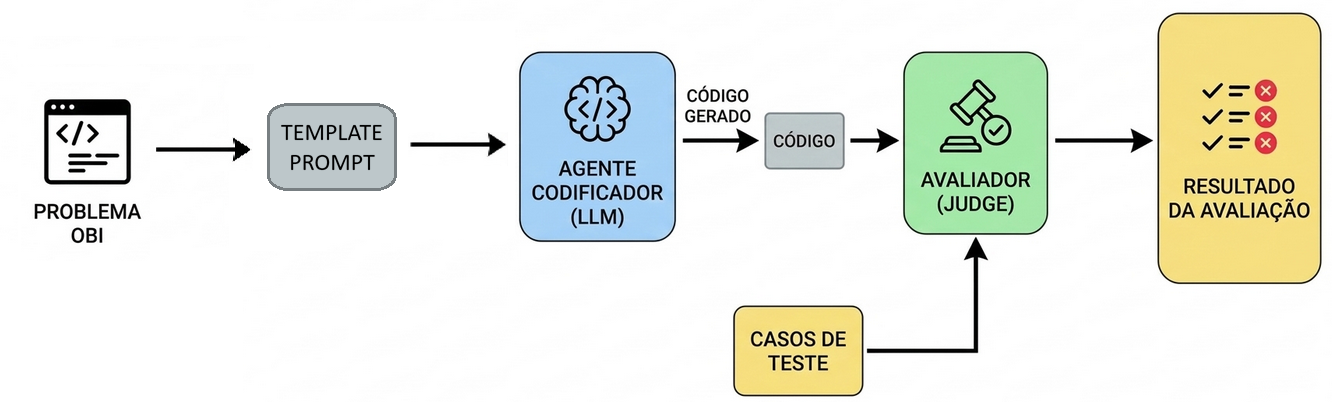
\includegraphics[width=\linewidth]{figures/1.png}
\caption{System pipeline}
\label{fig:pipeline}
\end{figure}

\subsection{Problem Dataset}\label{subsec:dataset}

To conduct the experiments, a problem dataset was built from the official website of the Brazilian Olympiad in Informatics (OBI). The compilation and structuring of this dataset were automated through a pipeline developed in Python, consisting of the following five steps:

\begin{itemize}
    \item \textbf{Data Collection (Web Scraping):} Download of the test booklets (covering all levels, from 2000 to 2025) using the \textit{requests} library to request page content and \textit{BeautifulSoup} to extract links.
    \item \textbf{Processing via LLM:} Submission of PDF files to the Gemini 3.1 Pro model for data extraction and structuring in JSON format. The generated fields included: title, statement, input, output, constraints, examples, score, year, level, period, and difficulty (the latter attribute inferred by the model itself). The exact prompt used for this extraction is detailed in Appendix \ref{apx:prompts}.
    \item \textbf{Test Case Obtainment:} Download of official answer keys (.zip files) corresponding to each question to extract expected inputs and outputs.
    \item \textbf{File Mapping:} Organization and linking of extracted test cases to their respective problems in the automatic judge directory.
    \item \textbf{Cleaning and Validation:} Removal of residual files and summary exclusion of questions that did not have an exact match with the input and output files, ensuring integrity for evaluation in the judge.
\end{itemize}

After consolidating the database, an exploratory analysis of the dataset was performed, classifying the problems under two main criteria: (i) difficulty level (easy, medium, and hard); and (ii) algorithmic domain, covering topics such as graphs, dynamic programming, greedy algorithms, and string processing, among others \cite{obi2026}.

At the end of the process, a manual analysis was performed to ensure the correctness of the answer keys and to add the images of the respective questions. Thus, the problem dataset obtained a validated sample of 493 questions in JSON format \cite{anonimo2026}.

\subsection{Evaluated Models}\label{subsec:models}

The experiments were conducted using different multimodal language models, which are capable of generating programming code from textual descriptions and images. The initial selection of the used models (Claude Sonnet 4.6, Gemini 3.1 Pro, GPT 5.4, Mistral Small 4, Grok 4.20) aimed to evaluate the impact of problem statement images on code generation. Subsequently, a second selection of models (Claude Sonnet 4.6, Gemini 3.1 Pro, GPT 5.4, DeepSeek-V3.2, Glm 5, Step 3.5 Flash, Grok Code Fast 1, and Mistral Small 4) was performed with the objective of verifying different architectural approaches, reflecting not only visual understanding but the current general landscape of generative artificial intelligence applied to competitive programming.

\subsection{Evaluation Environment}\label{subsec:evaluation}

An automated experimental environment was developed, responsible for managing the entire evaluation process of the solutions generated \cite{obibenchmarking2026} by the models. The environment performs the following steps during execution: choice of output environment; execution of a specific year for OBI questions; selection of a problem from the database in JSON format; sending the statement to the language model; receiving the generated code; compilation and execution of the code; and automatic evaluation using the test cases.

The verification of solutions is performed by comparing the output produced by the AI model's program and the expected output defined in the problem's test cases (Judge). Each solution is classified according to categories common in automatic judge systems, such as:

\begin{itemize}
    \item \textbf{Accepted (AC):} correct solution;
    \item \textbf{Wrong Answer (WA):} incorrect output;
    \item \textbf{Compilation Error (CE):} compilation error;
    \item \textbf{Runtime Error (RE):} error during execution;
    \item \textbf{Time Limit Exceeded (TLE):} exceeded time limit.
\end{itemize}

Since the problem booklets do not specify the execution time limit for the tests, the test cases were standardized to 1 second for the C++ language and to 3 seconds for the Python language. This difference is due to the paradigms in which both languages are inserted in the computational context. While the C++ language has its execution time optimized due to the use of a compiler, Python is executed line by line. Thus, in the competitive programming scenario, interpreted languages have a higher time limit than compiled languages.

\section{Experiments}\label{sec:experiments}

The conduct of the experiments involved the orchestration of API calls to the LLMs using a pass@1, temperature equal to 0, with \textit{top\_p} and \textit{max\_tokens} kept at their default values so as not to restrict the output size. In addition, the process included submission to the automatic judge and measurement of the execution time of submitted solutions. The hardware environment used in these experiments consists of a 13th generation Intel Core i7-1360P processor (2.20 GHz), 16 GB of RAM (4800 MT/s), and integrated Intel Iris Xe graphics accelerator, operating under the Windows 11 Home (64 bits) system.

Thus, Section \ref{subsec:verif_images} and Section \ref{subsec:exp_prep} present a preliminary experiment conducted to determine the optimal generation settings. In this stage, the performance of multimodal models regarding the use of images was evaluated, as well as the performance of Python and C++ languages, and the effectiveness of prompting strategies (zero-shot versus few-shot), since the choice of these parameters directly and significantly affects the accuracy and efficiency results of the models evaluated in this study.

\subsection{Verification of Images in Statements}\label{subsec:verif_images}

Before starting the environment preparation, a verification of the multimodal models was necessary to understand the impact that images have on code generation. When the statement contains references to images, as exemplified in Fig. \ref{fig:representacao}, these are converted to Base64 format during the prompt construction. In this way, multimodal models can extract visual information that may influence code generation and, consequently, the success rate.

\begin{figure}[htbp]
\centering
\includegraphics[width=\linewidth]{figures/2.png}
\caption{Representation of the statement for LLM models}
\label{fig:representacao}
\end{figure}

With this, the problem dataset has 181 questions with images, being 67 easy, 81 medium, and 33 hard. By analyzing the codes generated by the models with the number of correct answers according to the judge, it is visible that there was no significant gain in ACs.

\begin{table}[htbp]
\centering
\caption{Statistics of statements with and without images}
\label{tab:tabela1}
\resizebox{\linewidth}{!}{
\begin{tabular}{|l|c|c|c|c|c|c|}
\hline
\textbf{Model} & \textbf{Easy AC (With)} & \textbf{Easy AC (Without)} & \textbf{Medium AC (With)} & \textbf{Medium AC (Without)} & \textbf{Hard AC (With)} & \textbf{Hard AC (Without)} \\
\hline
Claude Sonnet 4.6 & 83.58\% & 77.61\% & 71.60\% & 74.07\% & 30.30\% & 36.36\% \\
GPT 5.4 & 82.09\% & 80.60\% & 69.14\% & 67.90\% & 30.30\% & 27.27\% \\
Gemini 3.1 Pro & 97.01\% & 97.01\% & 87.65\% & 87.65\% & 78.79\% & 75.76\% \\
Grok 4.20 & 73.13\% & 61.19\% & 53.09\% & 53.09\% & 15.15\% & 18.18\% \\
Mistral Small 4 & 61.19\% & 58.21\% & 41.98\% & 48.15\% & 12.12\% & 9.09\% \\
\hline
\end{tabular}
}
\end{table}

Furthermore, a considerable increase in code generation time was noted, as well as higher token consumption and increased average prompt cost. For this reason, the final experiment configuration adopts only texts, since, as illustrated in Table \ref{tab:tabela1}, there are no guarantees that providing images produces a substantial positive impact on the quality of the generated code.

\subsection{Experiment Environment Preparation}\label{subsec:exp_prep}

Using only the statements, the experiment seeks to verify simple prompt techniques such as zero-shot and few-shot for a better understanding of the models' performance for basic prompt techniques, attempting to solve 299 questions from the problem dataset, being 126 easy, 118 medium, and 55 hard. Because of this, in Kaplan et al. (2020) \cite{kaplan2020scaling}, scaling laws for language models were established, demonstrating that increasing parameters and computational power positively impacts overall performance. From this scalability, few-shot learning capabilities became viable in LLMs. However, Touvron et al. (2023) \cite{touvron2023llama} brought a new perspective with the development of LLaMA, showing that excellence in reasoning tasks (both in few-shot and zero-shot) does not depend exclusively on a massive scale of parameters, but on optimized training with a substantially larger volume of data.

In the preliminary experiment of this study, these dynamics were observed in practice. It was found that the zero-shot approach presented frequent failures in the strict input and output formatting required by the automatic judge in the OBI 2015 questions. To mitigate this problem, the few-shot technique was adopted by providing three problem examples (involving graphs, simple addition, and matrix counting) to guide the coding agent. This behavior is consistent with the reviewed literature \cite{brown2020language}: the models used in this benchmark have sufficient architectural capacity to infer patterns from the prompt examples, significantly improving the understanding of the I/O (input/output) format before generating the solution, as illustrated in Fig. \ref{fig:fewshot}.

\begin{figure}[htbp]
\centering
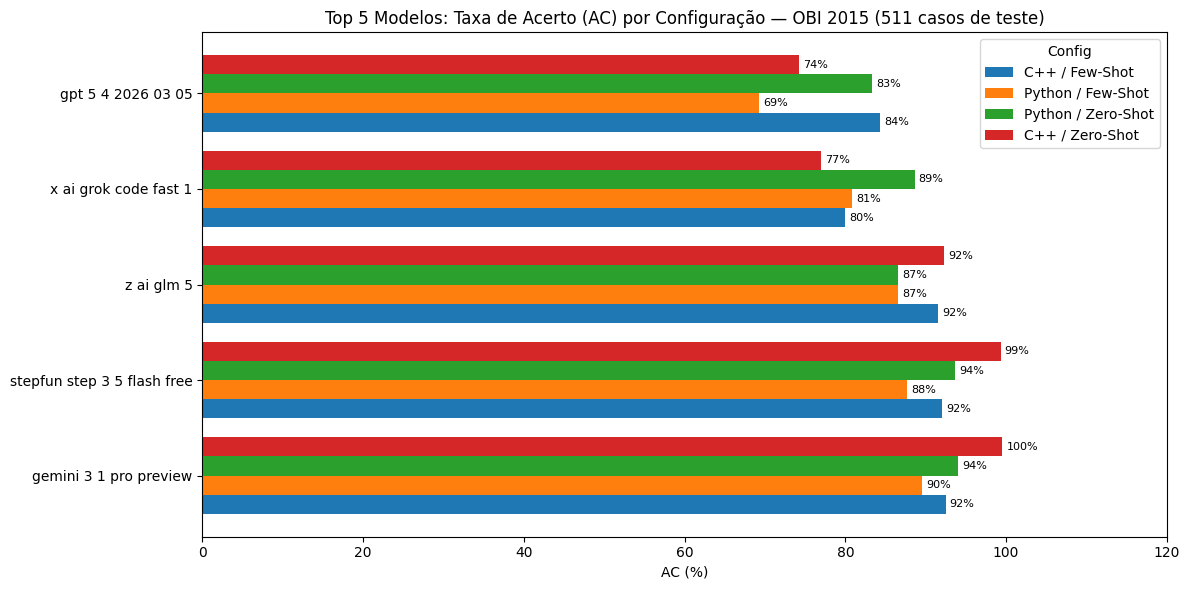
\includegraphics[width=\linewidth]{figures/4.png}
\caption{Top 5 test case success rates in the judge relative to programming language and prompt engineering technique}
\label{fig:top5}
\end{figure}

It should be noted that this preliminary experiment evaluated 511 test cases. The configuration that obtained the best performance among the top five evaluated models was the use of the Python language combined with the ``few-shot'' technique. Consequently, this was the methodological configuration adopted for the main evaluation of the present article.

\subsection{Evaluation Metrics}\label{subsec:metrics}

For the evaluation of the models' performance against the database composed of 299 OBI questions, metrics were defined to measure both algorithmic resolution efficacy and computational and financial efficiency. The comparative analysis is based on the following indicators:

\begin{itemize}
    \item \textbf{Success Rate (Accuracy):} Proportion of solutions that obtained full approval in all automatic judge test cases, stratified by the three problem difficulty levels.
    \item \textbf{Token Consumption:} Average of trafficked tokens (summing the input prompt and the generated solution) per problem.
    \item \textbf{API Cost:} Estimate of the average financial expenditure per request for code generation.
    \item \textbf{Inference Latency:} Average time elapsed for the complete generation of the code by the model.
\end{itemize}

\section{Results and Discussions}\label{sec:results}

\subsection{Performance Overview}\label{subsec:perf_overview}

This section presents a global analysis of the results obtained in the submission of the 299 questions to the automatic judge. The objective of this initial survey is to provide an overview of the actual capabilities and limitations of the evaluated tools, considering not only the absolute success rate but also the practical feasibility in terms of latency and financial cost.

The evaluation of the 299 questions revealed that part of the models failed to generate syntactically valid codes, a phenomenon observed predominantly in hard-level problems. This result shows that the high algorithmic complexity inherent to competitive programming still represents a substantial barrier to the capacity of executable code synthesis by these tools.

\begin{table}[htbp]
\centering
\caption{Experiment execution statistics}
\label{tab:tabela2}
\resizebox{\linewidth}{!}{
\begin{tabular}{|l|c|c|c|c|}
\hline
\textbf{Model} & \textbf{Total Tokens} & \textbf{Resolution Time} & \textbf{Total Cost} & \textbf{Outputs Without Code} \\
\hline
DeepSeek V3.2 & 544,573 & 1h 32m 26s & U\$ 0.21 & 0 \\
GLM 5 & 2,388,250 & 9h 42m 31s & U\$ 6.72 & 10 \\
GPT 5.4 & 457,127 & 0h 16m 5s & U\$ 1.98 & 0 \\
Gemini 3.1 Pro & 520,516 & 4h 35m 28s & U\$ 1.86 & 0 \\
Grok Code Fast 1 & 2,116,256 & 1h 59m 45s & U\$ 2.58 & 4 \\
Mistral Small 4 & 506,877 & 0h 9m 59s & U\$ 0.11 & 0 \\
Sonnet 4.6 & 877,409 & 1h 33m 42s & U\$ 7.22 & 0 \\
Step 3.5 Flash Free & 4,239,921 & 10h 8m 2s & U\$ 1.65 & 19 \\
\hline
\end{tabular}
}
\end{table}

Additionally, the analysis indicated the absence of a direct correlation between inference cost and algorithmic performance in the automatic judge (judge). Higher financial cost models did not necessarily present the highest success rates. In this context, according to the data in Table \ref{tab:tabela2}, the GPT 5.4 and Grok Code Fast 1 models stood out for their low latency, configuring themselves as suitable and agile options for solving easy and medium-level problems.

\begin{figure}[htbp]
\centering
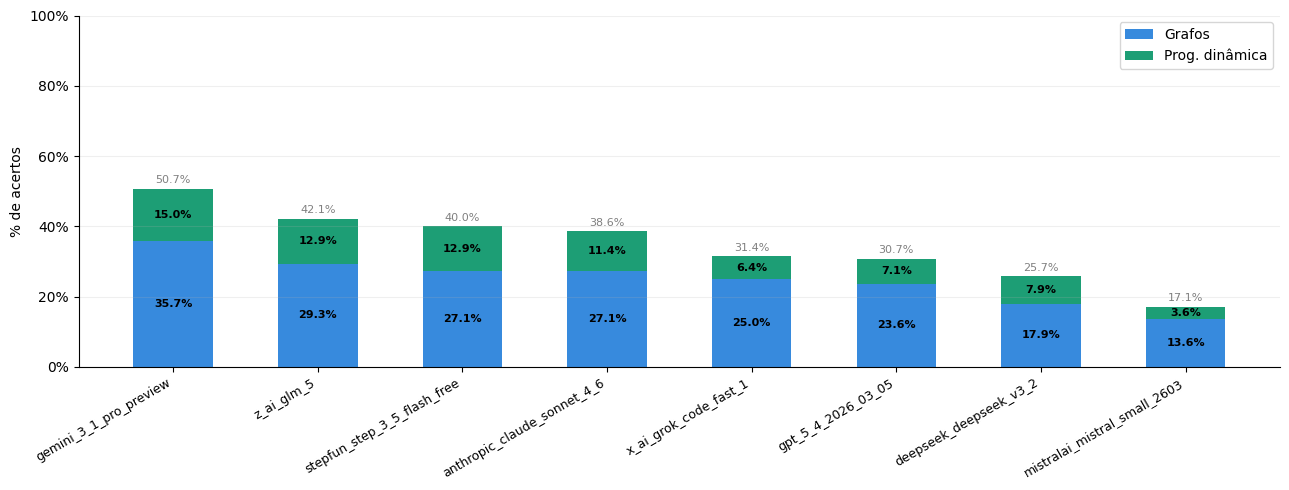
\includegraphics[width=\linewidth]{figures/6.png}
\caption{Success rate in dynamic programming and graphs topics}
\label{fig:topicos}
\end{figure}

It is noted that for graph and dynamic programming problems, the models' performance was substantially lower. Since only the Gemini 3.1 Pro model obtained a success rate of 50.70\%, it consolidates itself as the most recommended model to deal with these specific topics.

\begin{table}[htbp]
\centering
\caption{Benchmarking LLM models solving questions}
\label{tab:tabela3}
\resizebox{\linewidth}{!}{
\begin{tabular}{|l|c|c|c|c|c|c|}
\hline
\textbf{Model} & \textbf{Easy AC (\%)} & \textbf{Medium AC (\%)} & \textbf{Hard AC (\%)} & \textbf{Tokens (Avg)} & \textbf{Avg Cost (US\$)} & \textbf{Avg Time (s)} \\
\hline
DeepSeek V3.2 & 90.48 & 72.88 & 27.87 & 1785 & 0.0007 & 18 \\
GLM 5 & 90.48 & 83.90 & 50.82 & 7830 & 0.0220 & 115 \\
GPT 5.4 & 84.92 & 64.41 & 36.07 & 1499 & 0.0065 & 3 \\
Gemini 3.1 Pro & 92.86 & 89.83 & 72.13 & 1707 & 0.0061 & 54 \\
Grok Code Fast 1 & 87.30 & 70.34 & 34.43 & 6939 & 0.0085 & 24 \\
Mistral Small 4 & 60.32 & 44.07 & 13.11 & 1662 & 0.0004 & 2 \\
Sonnet 4.6 & 84.92 & 77.97 & 42.62 & 2877 & 0.0237 & 18 \\
Step 3.5 Flash Free & 92.06 & 83.05 & 55.74 & 13901 & 0.0054 & 120 \\
\hline
\end{tabular}
}
\end{table}

Finally, the Gemini 3.1 Pro model demonstrated the best cost-benefit ratio of the experiment. The tool reached the highest overall success rates in the judge, maintaining a competitive average cost compared to models like Claude Sonnet 4.6 and GLM 5. Its only significant limitation was latency, registering the third-highest average generation time per problem. In contrast, the Mistral Small 4 model presented the lowest performance of the study. On the opposite spectrum, the Step 3.5 Flash Free model stood out positively by achieving success rates comparable or superior to those of paid commercial models, despite operating with a reduced architecture of 11 billion active parameters.

\subsection{Success Rate by Difficulty Levels}\label{subsec:success}

The coding agents had a performance considered high for easy questions (above 81\%, except Mistral Small 4) and medium (above 59\%, except Mistral Small 4), because they are less complex problems that frequently do not require advanced input preprocessing or require the application of only a basic programming technique to reach the expected output.

However, since LLMs still have some difficulty in achieving full coverage in hard questions, it shows that seeking knowledge in LLMs is not guaranteed to answer the question, especially for competitive programming questions. Thus, structured interventions to deal with complex concepts, requiring targeted pedagogical approaches for each student profile \cite{baist2017analysis}, are strictly necessary when integrating Artificial Intelligence into education.

Therefore, this scenario is evidenced by the performance data of the Claude Sonnet 4.6 model itself, which, although reaching success rates of 84.92\% and 77.97\% in easy and medium-level problems, suffers an abrupt drop to only 42.62\% in hard questions. This demonstrates that Artificial Intelligence is evolving in transitioning from basic syntax to complex algorithmic reasoning, but caution is needed.

\section{Conclusion}\label{sec:conclusion}

This article presented a comprehensive experimental evaluation of the capability of different Large Language Models (LLMs) in solving programming problems, using the Brazilian Olympiad in Informatics (OBI) as a benchmark. The automated environment developed allowed quantifying not only the syntactic correctness of the generated code but also the logical and algorithmic efficacy against rigorous test cases.

The results demonstrate that models such as GLM 5, Sonnet 4.6, Step 3.5 Flash Free, GPT 5.4, and DeepSeek V3.2 present mastery in basic and intermediate-level problems. However, there is a sharp degradation in performance in questions requiring complex algorithmic reasoning, specifically in graphs and dynamic programming. This difficulty can be attributed to the autoregressive generation mechanism of LLMs: by producing an output token by token, from left to right, the model has limitations in backtracking and correcting complex logic previously built in the same iteration. Furthermore, the linearity of code generation directly impacts the occurrence of compilation errors and problems in time and memory management.

The investigation also revealed that the multi-agent approach, observed in the Grok Code Fast 1 model, outperformed single-agent configurations in initial exploration scenarios. For OBI competitive programming problems, single-agent-based models make more coding errors due to the large length of the statements, the requirement for deep logical reasoning, and the need for absolute syntactic rigor. The division of the problem into specialized sub-agents, a mechanism adopted by Grok Code Fast 1, manages to optimize these steps and achieves a success rate of 92.06\% in easy-level questions. On the other hand, Gemini 3.1 Pro Preview stood out for its technical consistency in overall resolution, especially with the Python language. It was also shown that the use of few-shot prompting acts as an essential strategy to mitigate I/O formatting errors, even though the increased context may introduce additional latency in the inference process (see Appendix \ref{apx:fewshot_examples} for the specific formatting examples provided to the models).

Ultimately, this study reaffirms that, despite the potential of LLMs as support tools, human expertise in competitive programming remains indispensable. Because current models exhibit significant constraints in deep logical reasoning and strict formatting adherence, they are not yet suited to act as fully autonomous solvers of complex algorithmic problems. Instead, their true potential in education lies in their architectural integration as interactive, intelligent tutoring bots. By employing strategies such as multi-agent orchestration, few-shot prompting, and dynamic knowledge tracing, future smart education systems can leverage generative LLMs to mediate the learning process, providing personalized guidance, dynamic hints, and real-time feedback, rather than simply generating direct final answers. Recent empirical studies corroborate this vision; for example, Peng et al. \cite{peng2025enhancing} demonstrated that systems coupling LLMs with code assistants and dynamic feedback significantly outperform traditional methods in both learning gains and problem-solving accuracy.

As a development of this research, it is proposed to expand the experimental evaluation to an olympiad question bank with a wider variety of problems and different styles, such as the initiation modality, and to actively develop intelligent tutor prototypes based on the architectural findings of this study.

\appendices

\section{Prompt Templates}
\label{apx:prompts}

This appendix presents the English translation of the prompt templates used in this study to interact with the Large Language Models.

\subsection{Problem Extraction Prompt}
The following prompt was used to extract competitive programming problems from the official PDF booklets and structure them into JSON format.

\begin{tcolorbox}[breakable, colframe=black!75, colback=black!5, title=\textbf{Prompt: Problem Extractor}]
\textbf{\#\#\# PERSONA \#\#\#}\\
You are an expert assistant specialized in extracting competitive programming problems from Brazilian Olympiad in Informatics (OBI) PDFs.

\textbf{\#\#\# TASK \#\#\#}\\
Read the attached PDF file and extract the data of ALL the problems you find in the document.
Return the data STRICTLY in the JSON format below, filling it with the document's information.

\textbf{\#\#\# RESTRICTIONS \#\#\#}\\
Your response must be an ARRAY (list) of JSON objects, where each object represents a different problem.
Do not include any markdown formatting (such as \texttt{```json}) or text before/after the JSON.

\textbf{EXPECTED TEMPLATE:}\\
\texttt{[\{}\\
\texttt{~~"title": "Problem name 1",}\\
\texttt{~~"statement": "Complete text of the problem description...",}\\
\texttt{~~"input": "Text of the Input section",}\\
\texttt{~~"output": "Text of the Output section",}\\
\texttt{~~"constraints": "Text of the Constraints section",}\\
\texttt{~~"examples": [\{"input": "...", "output": "..."\}],}\\
\texttt{~~"imgs": [],}\\
\texttt{~~"rating": [int: subtask 0 score, ...],}\\
\texttt{~~"year": "2024",}\\
\texttt{~~"level": "PJ",}\\
\texttt{~~"period": "Phase 3",}\\
\texttt{~~"topics": ["array", "graphs"],}\\
\texttt{~~"difficulty": "Hard"}\\
\texttt{\}]}
\end{tcolorbox}

\subsection{Code Generation Prompts}
Two distinct prompting strategies were applied to the coding agents: Zero-Shot and Few-Shot.

\begin{tcolorbox}[breakable, colframe=black!75, colback=black!5, title=\textbf{Prompt: Zero-Shot Code Generation}]
\textbf{\#\#\# PERSONA \#\#\#}\\
You are an experienced \texttt{\{language\}} developer specialized in competitive programming (OBI).

\textbf{\#\#\# TASK \#\#\#}\\
Your task is to read the problem description (the \texttt{[x.png]} tag is associated with a base64 format image, if not present ignore it), input and output descriptions, and examples, and generate ONLY the \texttt{\{language\}} code to solve it.

\textbf{\textless{}problem\_context\textgreater{}}\\
\texttt{\{context\}}\\
\textbf{\textless{}/problem\_context\textgreater{}}

\textbf{\#\#\# CRITICAL INSTRUCTIONS \#\#\#}
\begin{enumerate}
    \item The generated code must read from standard input and write to standard output.
    \item GENERATE ONLY CODE. Do not say anything. Do not reply with "Here is the code". Do not use extra Markdown blocks. Start directly with the libraries/imports.
    \item Ensure the code passes the time and memory constraints.
    \item The code must be valid and executable \texttt{\{language\}}.
\end{enumerate}
\end{tcolorbox}

\begin{tcolorbox}[breakable, colframe=black!75, colback=black!5, title=\textbf{Prompt: Few-Shot Code Generation}]
\textbf{\#\#\# PERSONA \#\#\#}\\
You are a World-Class OBI/ICPC Competitor, expert in \texttt{\{language\}}. Your mission is to write robust, high-performance code that passes 100\% of the test cases (including edge cases).

\textbf{\#\#\# TASK \#\#\#}\\
Generate the complete \texttt{\{language\}} code to solve the problem strictly based on the \textbf{\textless{}problem\_context\textgreater{}}. Note that the \texttt{[x.png]} tag is associated with a base64 format image; if not present, ignore the tags.

\textbf{\textless{}problem\_context\textgreater{}}\\
\texttt{\{context\}}\\
\textbf{\textless{}/problem\_context\textgreater{}}

\textbf{\#\#\# FORMAT REFERENCE EXAMPLES \#\#\#}\\
\texttt{\{examples\}}

\textbf{\#\#\# MANDATORY TECHNICAL GUIDELINES \#\#\#}
\begin{enumerate}
    \item \textbf{ANALYZE CONSTRAINTS:} Observe the limits of N and M in the context. Choose an algorithm with compatible time complexity.
    \item \textbf{DATA TYPES:} 
    \begin{itemize}
        \item If C++, use \texttt{long long} for values that might exceed $2 \times 10^9$.
        \item If Python, use \texttt{sys.stdin.read().split()} for fast I/O and \texttt{sys.setrecursionlimit(200000)} for recursion.
    \end{itemize}
    \item \textbf{OUTPUT FORMAT:} The output must be EXACTLY as requested. Pay attention to extra spaces and line breaks.
    \item \textbf{ZERO EXPLANATION:} Do not say anything. Do not reply with "Here is the code". Do not use extra Markdown blocks. Start directly with the libraries/imports.
\end{enumerate}
\end{tcolorbox}

\subsection{Few-Shot I/O Formatting Examples}
\label{apx:fewshot_examples}

In the Few-Shot setting, providing language-specific input and output examples is crucial to improve the accuracy of the automated judge. These examples explicitly guide the model to adopt strict I/O conventions, such as fast bulk reading in Python and optimized streams in C++, significantly mitigating parsing failures, runtime exceptions, and Time Limit Exceeded (TLE) errors during the evaluation process.

\begin{tcolorbox}[breakable, colframe=black!75, colback=black!5, title=\textbf{Python I/O Examples}]
\textbf{Example 1 (Problem: Sum of two numbers)}\\
\textbf{\textless{}context\textgreater{}}\\
Write a program that reads two integers and prints the sum.\\
\textbf{\textless{}/context\textgreater{}}\\
\textbf{Expected response:}
\begin{verbatim}
import sys
a, b = map(int, sys.stdin.read().split())
print(a + b)
\end{verbatim}

\vspace{0.3cm}
\textbf{Example 2 (Problem: Count occupied cells)}\\
\textbf{\textless{}context\textgreater{}}\\
Given a grid of N rows and M columns, count how many '1' characters exist.\\
\textbf{\textless{}/context\textgreater{}}\\
\textbf{Expected response:}
\begin{verbatim}
import sys

input_data = sys.stdin.read().split()
if not input_data:
    exit()

n = int(input_data[0])
m = int(input_data[1])
grid = input_data[2:]

count = 0
for row in grid:
    count += row.count('1')

print(count)
\end{verbatim}
\end{tcolorbox}

\begin{tcolorbox}[breakable, colframe=black!75, colback=black!5, title=\textbf{C++ I/O Examples}]
\textbf{Example 1 (Problem: Sum of two numbers)}\\
\textbf{\textless{}context\textgreater{}}\\
Write a program that reads two integers and prints the sum.\\
\textbf{\textless{}/context\textgreater{}}\\
\textbf{Expected response:}
\begin{verbatim}
#include <bits/stdc++.h>
using namespace std;
int main() {
    int a, b;
    if (cin >> a >> b)
        cout << a + b << endl;
    return 0;
}
\end{verbatim}

\vspace{0.3cm}
\textbf{Example 2 (Problem: Count occupied cells)}\\
\textbf{\textless{}context\textgreater{}}\\
Given a grid of N rows and M columns, count how many '1' characters exist.\\
\textbf{\textless{}/context\textgreater{}}\\
\textbf{Expected response:}
\begin{verbatim}
#include <bits/stdc++.h>
using namespace std;

int main() {
    ios::sync_with_stdio(0);
    cin.tie(0);

    int n, m;
    if (!(cin >> n >> m)) return 0;

    int count = 0;
    for (int i = 0; i < n; i++) {
        string row;
        cin >> row;
        for (char c : row) {
            if (c == '1') count++;
        }
    }

    cout << count << endl;
    return 0;
}
\end{verbatim}
\end{tcolorbox}

\bibliographystyle{IEEEtran}
\bibliography{references}

\end{document}
